% Subsection on audio amplifier

Un \emph{amplificateur audio} est nécessaire pour pouvoir ressortir le son sur un baffle ou un buzzer. Pour cela, on a à disposition des circuits intégrés à 14 pattes (modèle LM380N de chez Texas Instruments). Le chip LM380N choisi est montré en photo sur la Figure \ref{fig:ampli_pic}.\\

Le sens du boîtier de l'amplificateur est renseigné avec une petite encoche, généralement placée vers le haut. Chaque patte/pin du circuit a un but précis et un nom, renseigné sur la Figure \ref{fig:ampli_pins}. Par exemple, le circuit est alimenté avec du +15V, à connecter sur sa pin 14 ($V_s$). La masse ou 0V, aussi nommée $GND$, doit être connectée à plusieurs pins (3, 4, 5, 7, 10, 11, 12), notamment pour une question de dissipation de puissance. Il ne faut pas oublier qu'il s'agit d'un amplificateur audio qui nécessite quand même un peu de puissance. Les autres connexions sont à retrouver sur le schéma général du circuit à la Figure \ref{fig:schematics}.\\

\begin{minipage}[c]{.49\textwidth}
	\centering
	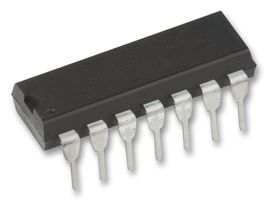
\includegraphics[width=0.6\textwidth]{figures/LM380N_picture.jpg}
	\captionof{figure}{Photo de l'amplificateur audio LM380N.}
	\label{fig:ampli_pic}
\end{minipage}
\hfill
\begin{minipage}[c]{.49\textwidth}
	\centering
	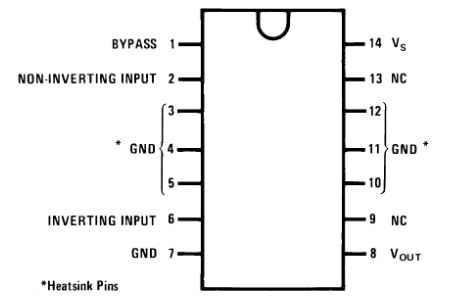
\includegraphics[width=\textwidth]{figures/LM380N_sch.jpg}
	\captionof{figure}{Nom des pattes de l'amplificateur audio LM380N.}
	\label{fig:ampli_pins}
\end{minipage}
\vspace{1cm}